% Research Note 01 -- Seasonal structure and residual modeling of CA highway traffic flow
% Compile with any standard LaTeX engine, e.g.:
%   pdflatex note01_seasonal_baseline.tex   (run twice for refs)
% Requires the PNGs in ./figures/ (produced by src/eda.py and src/residual_acf.py).
\documentclass[11pt]{article}
\usepackage[margin=1in]{geometry}
\usepackage{amsmath,amssymb}
\usepackage{graphicx}
\usepackage{booktabs}
\usepackage{float}
\usepackage{xcolor}
\usepackage[colorlinks=true,linkcolor=blue,urlcolor=blue]{hyperref}
\graphicspath{{figures/}}

\newcommand{\veh}{\,\text{veh/h}}
\title{\textbf{Research Note 01}\\[2pt]
Seasonal Structure and Residual Modeling of\\ California Highway Traffic Flow}
\author{Traffic Forecasting Project}
\date{June 14, 2026}

\begin{document}
\maketitle

\begin{abstract}
\noindent
We study one-week-ahead ($H{=}168$ hourly) forecasting of freeway traffic
\emph{flow} in the Greater Bay Area, using five years of Caltrans loop-detector
data (LargeST). We show that a trivial \emph{seasonal baseline} -- the average
of the same hour-of-week over the previous four weeks -- explains roughly
$94\%$ of the variance of hourly flow, per cell (sensor $\times$ hour). We then
study the \emph{seasonal residual} $r=y-b$, establish that for a one-week-ahead
task only \emph{weekly} lags are usable, and evaluate a seasonal autoregression
on the residual. It yields a small but consistent out-of-sample gain
($\sim$3\% RMSE), and its fitted coefficients reveal that the real signal is a
\emph{re-weighting} of the flat four-week average toward more recent weeks. We
close with concrete next steps.
\end{abstract}

\section*{Key findings}
\begin{itemize}
\item Traffic \textbf{volume} is dominated by a strong, stable weekly cycle
  (commute peaks; weekday/weekend contrast).
\item A per-cell \textbf{4-week hour-of-week mean baseline} explains
  $\mathbf{>90\%}$ of variance: pooled $R^2 = 0.936$, per-sensor median
  $R^2=0.913$, stable across 2017--2019.
\item The \textbf{seasonal residual} has strong \emph{short}-lag autocorrelation
  (AR(1)-like, lag-1 $=0.81$) but only weak/negative \emph{weekly}-lag
  autocorrelation -- the latter partly an artifact of the baseline filter.
\item For \textbf{week-ahead} forecasting, short lags are unusable; only weekly
  lags are available across the whole horizon. A seasonal-residual AR on weekly
  lags gives $\sim$3\% RMSE improvement and, interpreted as weights on raw weekly
  values, \textbf{learns a decaying (EWMA-like) weekly average}.
\end{itemize}

\section{The dataset}
\label{sec:data}

\paragraph{Source.} The data come from the Caltrans Performance Measurement
System (PeMS), which aggregates measurements from inductive-loop detectors
embedded in the freeway pavement across California. Each \emph{station} (which we
also call a \emph{sensor} or \emph{spatial unit}) reports, in five-minute bins,
three quantities: \emph{flow} (vehicle count per unit time), \emph{occupancy}
(fraction of time the detector is covered by a vehicle), and \emph{speed}. We
forecast \textbf{flow}, the most directly seasonal of the three; speed is far
noisier (dominated by incident-driven congestion) and, in a parallel check on
the PeMS-BAY speed dataset, the same baseline reached only $R^2\approx0.76$
versus $0.94$ for flow.

\paragraph{Benchmark and region.} We use \textbf{LargeST} (Liu et al., NeurIPS
2023), which assembles $8{,}600$ PeMS sensors statewide at 5-minute resolution
for 2017--2021. We restrict to \textbf{Caltrans District 4 (Greater Bay Area)},
$N=2{,}352$ sensors, and -- to avoid the COVID-19 disruption -- use the
pre-pandemic years \textbf{2017--2019} as the working set. (2020 is cached
separately for a future stress test; LargeST ends in 2021, so genuinely
post-pandemic data would have to be pulled from the PeMS Clearinghouse.)

\paragraph{Aggregation and notation.} We average the 5-minute series to hourly
(12 bins $\to$ 1 hour). The result is a matrix
\[
Y \in \mathbb{R}^{T\times N},\qquad
y_{i,t} = \text{mean flow (\veh) at sensor } i \text{ during hour } t,
\]
with $T = 26{,}280$ hourly steps ($3$ years) and $N=2{,}352$ sensors. Each
sensor $i$ is a fixed location, freeway, and direction (e.g.\ I-80~W). A
typical sensor carries a median flow of $\sim$$220\veh$. Missing values
(NaN, $\sim$2\% of hours) are imputed per sensor with that sensor's hour-of-week
mean. We define the weekly period
\[
P = 24\times 7 = 168 \text{ hours},
\]
and the \emph{hour-of-week} index $\phi(t)=t \bmod P \in\{0,\dots,167\}$, which
encodes both the day-of-week and the hour-of-day of timestamp $t$.

\section{Exploratory analysis: a strong weekly cycle}
\label{sec:eda}

Figure~\ref{fig:profile} shows the mean flow as a function of hour-of-week for
three sensors (busy / median / quiet). The structure is striking and highly
regular: each weekday shows the classic \emph{double peak} (morning and evening
commutes); weekends collapse into a single broad midday hump; and the shape
repeats week after week. Figure~\ref{fig:heatmap} renders the same information
for one busy sensor as a day-of-week $\times$ hour-of-day heatmap.

\begin{figure}[H]
\centering
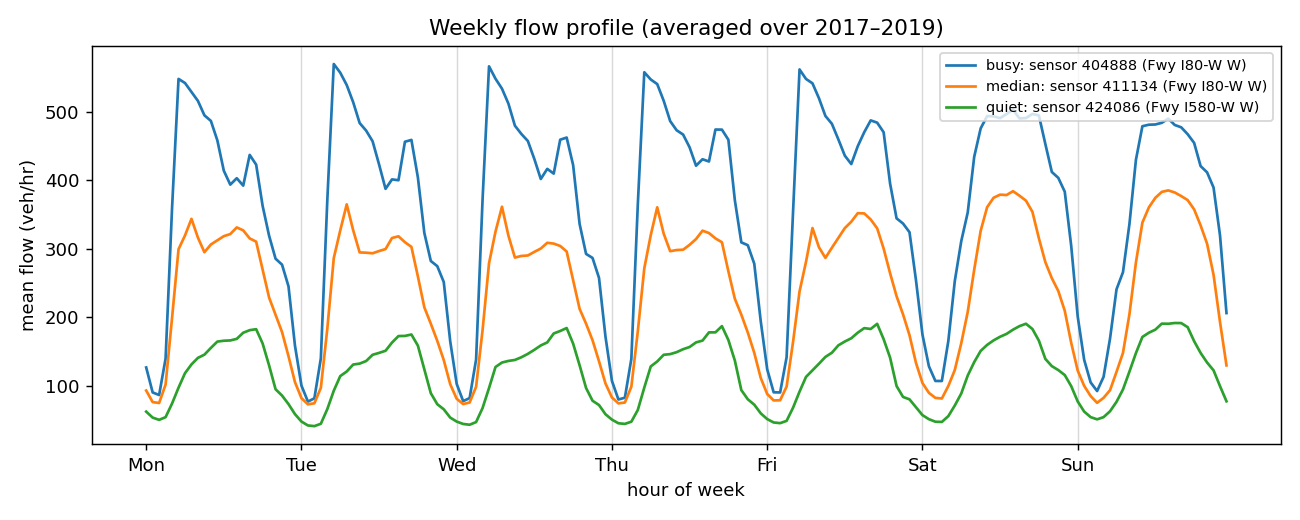
\includegraphics[width=\linewidth]{fig1_weekly_profile.png}
\caption{Mean flow by hour-of-week (averaged over 2017--2019) for three sensors.
Vertical lines mark day boundaries. Weekday commute double-peaks and the
weekend single-hump are visible and stable across all seven days.}
\label{fig:profile}
\end{figure}

\begin{figure}[H]
\centering
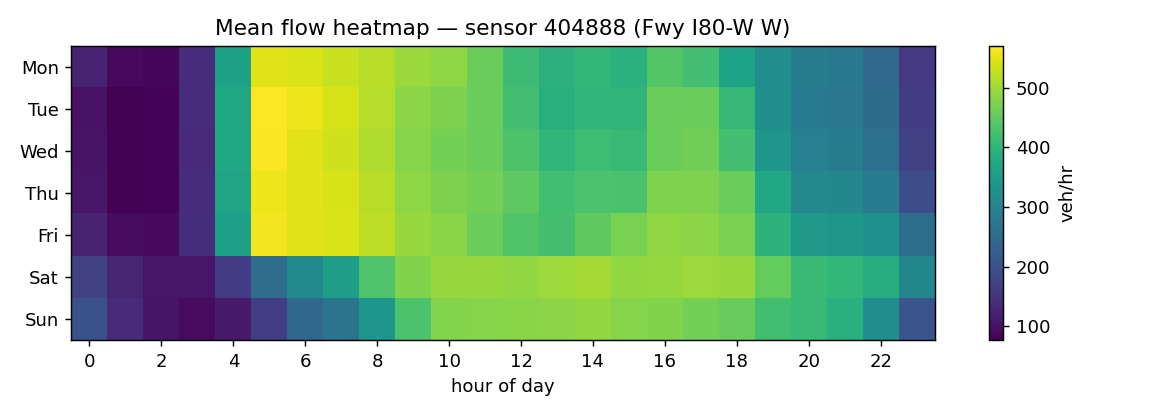
\includegraphics[width=0.85\linewidth]{fig2_heatmap.png}
\caption{Mean flow heatmap (weekday $\times$ hour-of-day) for a busy I-80~W
sensor. The bright morning/evening commute bands on weekdays and the diffuse
weekend pattern summarize the dominant seasonal signal.}
\label{fig:heatmap}
\end{figure}

\section{The seasonal baseline}
\label{sec:baseline}

Because the weekly cycle is so dominant, a natural predictor for any cell is the
recent average at the \emph{same hour of week}. We define the four-week
\textbf{seasonal baseline}
\begin{equation}
b_{i,t} \;=\; \frac{1}{4}\sum_{k=1}^{4} y_{i,\,t-Pk},
\qquad P=168.
\label{eq:baseline}
\end{equation}
Every lag is a multiple of one week, so $b_{i,t}$ averages the four most recent
realizations of the same hour-of-week.

\paragraph{It is a valid one-week-ahead forecast.} At a forecast origin $t$,
consider a target $s=t+h$ with horizon $h\in\{1,\dots,168\}$. Every term in
$b_{i,s}=\frac14\sum_{k=1}^4 y_{i,s-Pk}$ has index $s-Pk \le t$ for all $k\ge1$
(since $h\le P$). Hence the baseline for the \emph{entire} week ahead is known at
$t$ with \textbf{no leakage and no recursion}.

\paragraph{It explains $>90\%$ of variance.} Define the per-sensor variance
explained
\[
\mathrm{VE}_i = 1 - \frac{\operatorname{Var}_t(r_{i,t})}{\operatorname{Var}_t(y_{i,t})},
\qquad r_{i,t}=y_{i,t}-b_{i,t}.
\]
Pooled over all cells, $\mathrm{VE}=0.936$; the per-sensor distribution
(Figure~\ref{fig:vehist}) has median $0.913$ and 10th--90th percentiles
$[0.845,\,0.950]$. In a full rolling-origin backtest (origins stepped daily,
$H=168$, $1{,}061$ forecasts), the baseline attains the metrics in
Table~\ref{tab:baselines}, stable year to year ($R^2 = 0.941/0.928/0.940$ for
2017/2018/2019). Overall the baseline reduces the standard deviation of flow
from $164.6\veh$ to a residual $41.7\veh$ -- it removes about three-quarters of
the typical fluctuation.

\begin{table}[H]
\centering
\caption{Rolling-origin one-week-ahead backtest, GBA 2017--2019
($1{,}061$ weekly forecasts $\times\,2{,}352$ sensors).}
\label{tab:baselines}
\begin{tabular}{lccc}
\toprule
Forecaster & Pooled $R^2$ & RMSE (\veh) & Per-sensor median $R^2$ \\
\midrule
Hour-of-week mean, 4 weeks & 0.936 & 41.7 & 0.913 \\
Hour-of-week mean, 8 weeks & 0.937 & 41.2 & 0.915 \\
Same hour, last week only  & 0.910 & 49.5 & 0.878 \\
\bottomrule
\end{tabular}
\end{table}

\begin{figure}[H]
\centering
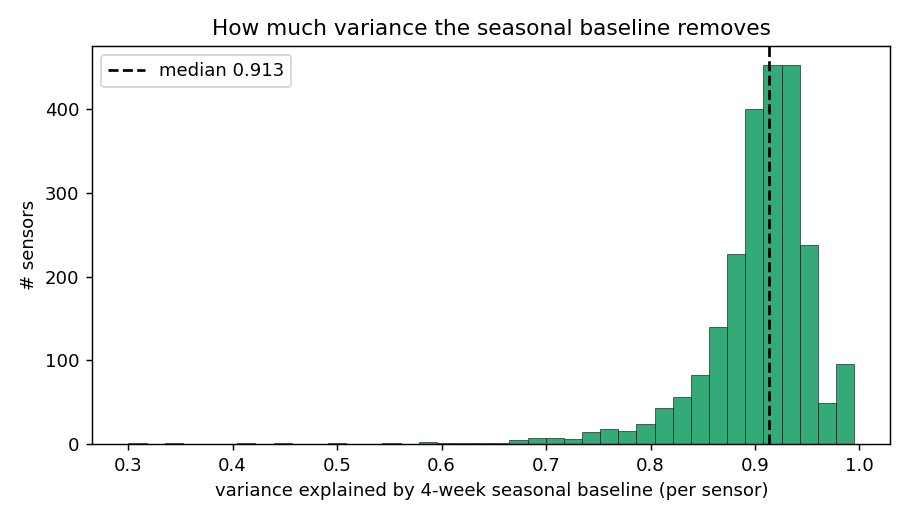
\includegraphics[width=0.7\linewidth]{fig3_ve_hist.png}
\caption{Distribution over sensors of variance explained by the 4-week seasonal
baseline. Even the hardest cells exceed $0.84$; there is no long unpredictable
tail (unlike speed).}
\label{fig:vehist}
\end{figure}

\section{The seasonal residual}
\label{sec:residual}

We now model what the baseline leaves behind, the \textbf{seasonal residual}
\begin{equation}
r_{i,t} \;=\; y_{i,t} - b_{i,t}
\;=\; \Big(1 - \tfrac14\textstyle\sum_{k=1}^{4} B^{Pk}\Big)\, y_{i,t},
\label{eq:residual}
\end{equation}
where $B$ is the backshift operator ($B^{m}y_t=y_{t-m}$). Equation
\eqref{eq:residual} makes explicit that the baseline is a \emph{seasonal filter}:
$r$ is $y$ with a weekly moving-average level removed. Figure~\ref{fig:decomp}
shows the decomposition for one sensor over three weeks; the baseline tracks the
shape tightly and the residual is the harder, irregular remainder.

\begin{figure}[H]
\centering
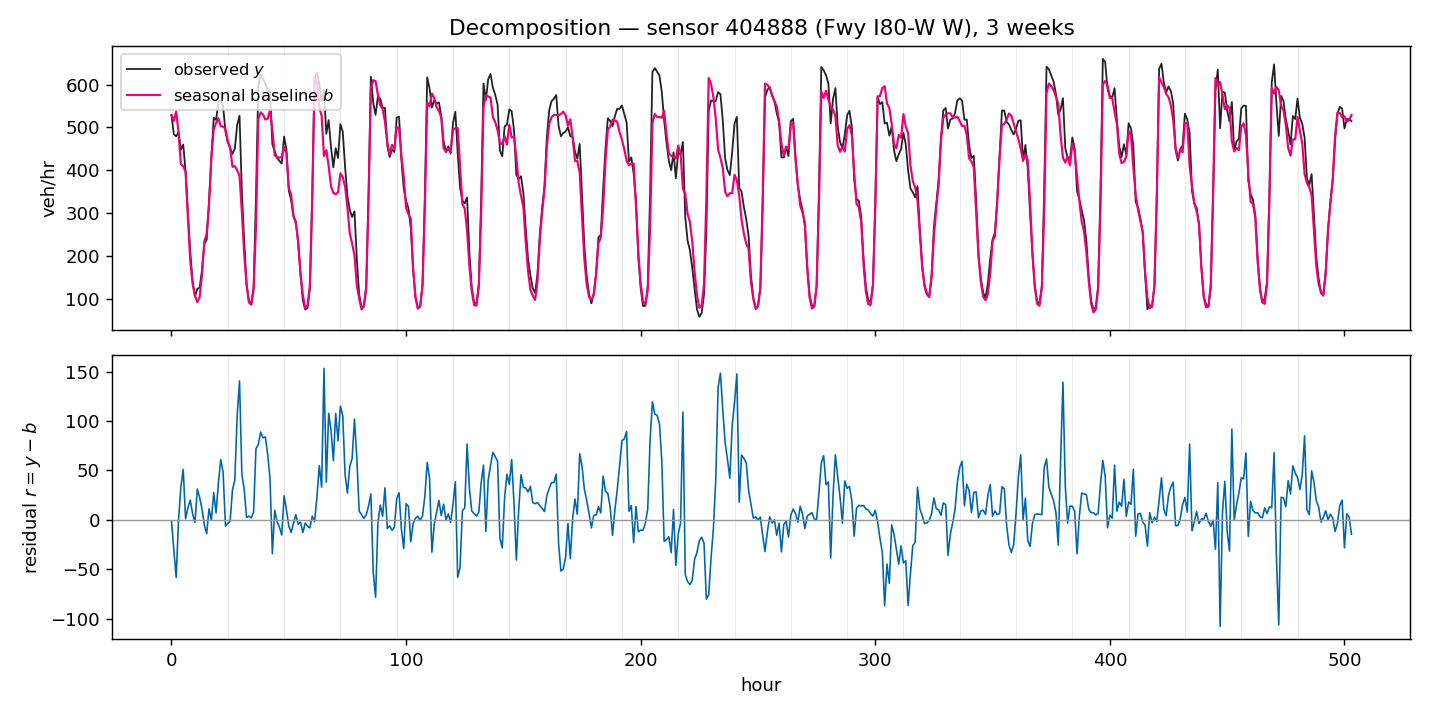
\includegraphics[width=\linewidth]{fig4_decomposition.png}
\caption{Top: observed flow $y$ and seasonal baseline $b$ for a busy sensor over
three weeks. Bottom: the residual $r=y-b$.}
\label{fig:decomp}
\end{figure}

\subsection{Autocorrelation structure}
Figure~\ref{fig:acf} and Table~\ref{tab:acf} summarize the mean residual
autocorrelation (over 250 sensors). Three observations:
\begin{enumerate}
\item \textbf{Short lags dominate and are nearly pure AR(1).} The ACF decays as
  $0.806^{\,k}$ for the first few hours ($0.806,0.650,0.525$) and the partial
  ACF cuts off after lag~1 ($+0.806$, then $\approx 0$). There is a secondary
  \emph{daily} echo (lag~24 $=0.331$).
\item \textbf{The weekly lag is weak} ($+0.094$ at lag~168).
\item \textbf{The 2--4 week lags are negative} ($-0.05,-0.15,-0.18$). This is
  \emph{not} physical: by construction \eqref{eq:residual} subtracts the previous
  four same-hour-of-week values, so $r_t$ is mechanically anti-correlated with
  those weeks. The negative weekly tail is the fingerprint of the baseline
  filter, not week-over-week signal.
\end{enumerate}

\begin{table}[H]
\centering
\caption{Mean residual autocorrelation at selected lags (250 sensors).}
\label{tab:acf}
\begin{tabular}{lcccccccc}
\toprule
Lag (h) & 1 & 2 & 3 & 24 & 48 & 168 & 336 & 504/672 \\
\midrule
ACF & $+0.806$ & $+0.650$ & $+0.525$ & $+0.331$ & $+0.215$ &
$+0.094$ & $-0.049$ & $-0.149/{-}0.181$ \\
\bottomrule
\end{tabular}
\end{table}

\begin{figure}[H]
\centering
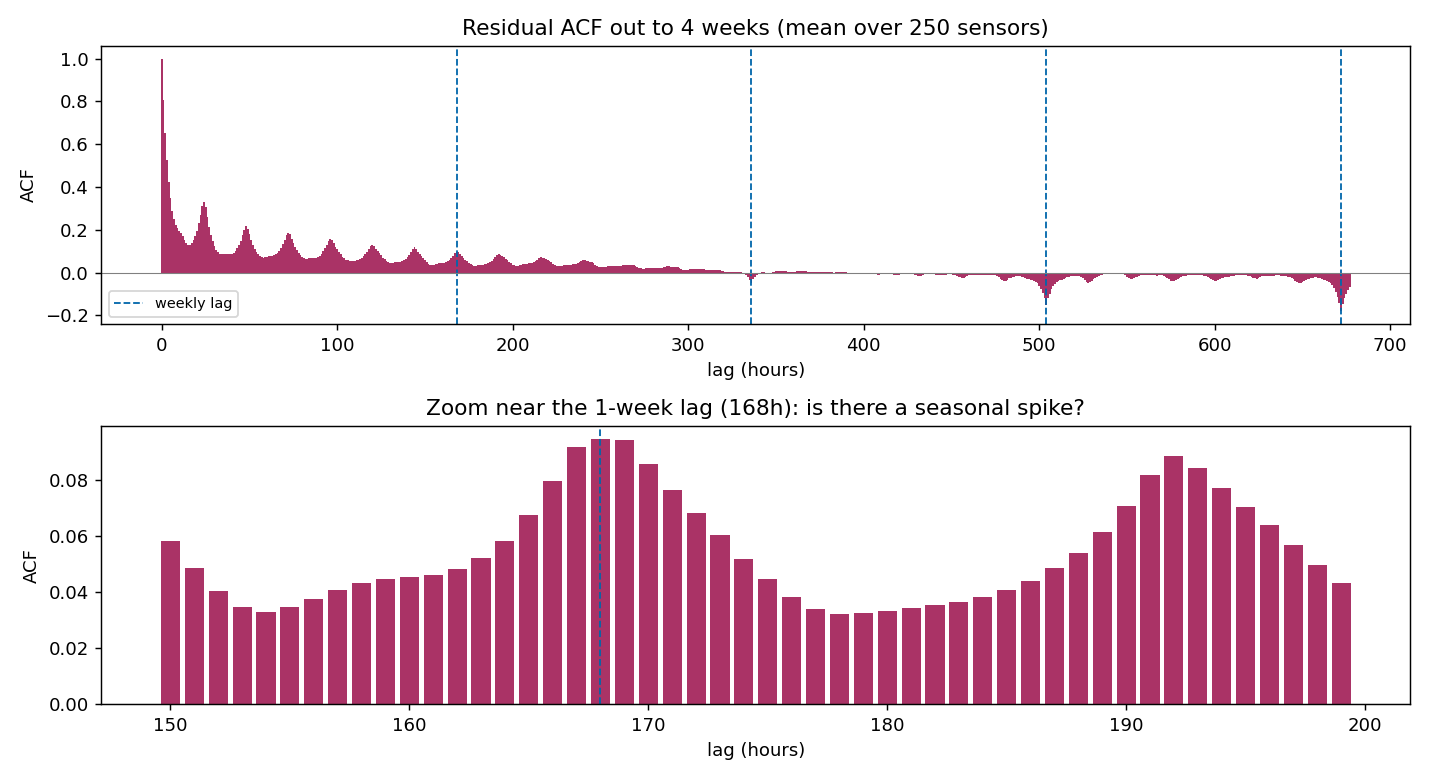
\includegraphics[width=\linewidth]{fig5_residual_acf.png}
\caption{Residual ACF out to four weeks (top) and zoomed near the one-week lag
(bottom). Dashed lines mark weekly lags. Note the daily echoes in the short-lag
region, the modest bump at $168$h, and the growing \emph{negative} values at
$2$--$4$ weeks induced by the baseline filter.}
\label{fig:acf}
\end{figure}

\section{Week-ahead constraint and the seasonal-residual AR}
\label{sec:model}

\paragraph{Why short lags are useless here.} The lag-1 autocorrelation of $0.81$
is irrelevant to a one-week-ahead forecast. At origin $t$, predicting target
$s=t+h$, the freshest usable observation is at $t$, i.e.\ $h$ hours before the
target; at the far end of the horizon ($h=168$) that is a \emph{full week}
before $s$. An hourly AR(1) iterated forward decays as $0.81^{h}\!\to\!0$ over
the week and contributes essentially nothing. \textbf{The only lags available
across the entire horizon are the weekly ones.}

\paragraph{Model.} We therefore model the seasonal residual from its own weekly
lags -- a seasonal autoregression:
\begin{equation}
\hat r_{i,s} \;=\; \psi_0 + \sum_{m=1}^{M}\psi_m\, r_{i,\,s-Pm},
\qquad
\hat y_{i,s} \;=\; b_{i,s} + \hat r_{i,s}.
\label{eq:sar}
\end{equation}
Crucially, each feature $r_{i,s-Pm}$ depends only on $y$ up to time $s-P\le t$,
so it is observed at the origin for \emph{every} horizon $h\in\{1,\dots,168\}$.
The model needs no recursion and applies uniformly across the horizon.

\paragraph{Out-of-sample result.} We fit \eqref{eq:sar} by pooled OLS on
2017--2018 and test on 2019 (Table~\ref{tab:sar}). The seasonal-residual AR gives
a small but consistent improvement ($\sim$3\% RMSE; residual $R^2\approx0.05$).
Two sharpenings of the picture:
\begin{itemize}
\item \textbf{A single weekly lag is essentially useless} (residual
  $R^2=0.004$). All the value comes from \emph{combining} weeks.
\item \textbf{The fitted coefficients are negative and growing,}
  \[
  \psi_1=+0.04,\quad \psi_2=-0.07,\quad \psi_3=-0.14,\quad \psi_4=-0.20,
  \]
  echoing the negative ACF tail.
\end{itemize}

\begin{table}[H]
\centering
\caption{Seasonal-residual AR, trained 2017--18, tested 2019
(pooled OLS, 600-sensor subsample). Baseline figures here differ slightly from
Table~\ref{tab:baselines} due to the single-split, subsampled setup.}
\label{tab:sar}
\begin{tabular}{lccc}
\toprule
Model & Residual $R^2$ & One-week-ahead $y$ $R^2$ & RMSE (\veh) \\
\midrule
Baseline only ($\hat r=0$)        & ---     & 0.9417 & 39.65 \\
\;+ seasonal-AR, 4 weekly lags    & $0.051$ & 0.9447 & 38.62 \ ($-2.6\%$) \\
\;+ seasonal-AR, 8 weekly lags    & $0.058$ & 0.9451 & 38.48 \ ($-3.0\%$) \\
\;1 weekly lag only               & $0.004$ & ---    & 39.56 \ ($-0.2\%$) \\
\bottomrule
\end{tabular}
\end{table}

\paragraph{Interpretation: the model is re-weighting the baseline.} Substituting
$r_{i,s-Pm}=y_{i,s-Pm}-b_{i,s-Pm}$ into \eqref{eq:sar}, the coefficient on the
raw weekly value $y_{i,s-Pm}$ becomes $\tfrac14+\psi_m$ for $m=1,\dots,4$ (plus
smaller corrections from weeks 5--8 carried by the $b_{i,s-Pm}$ terms). With the
fitted $\psi$ this gives effective weekly weights of approximately
\[
(0.29,\ 0.18,\ 0.11,\ 0.05)
\qquad\text{versus the flat}\qquad
(0.25,\ 0.25,\ 0.25,\ 0.25).
\]
In other words, the seasonal-residual AR is not exploiting
``last week's anomaly persists'' -- that signal is near zero. It is discovering
that \textbf{recent weeks deserve more weight than older ones}, i.e.\ it converts
the flat four-week mean into a \emph{decaying, EWMA-like} weekly average.

\section{Limitations}
\label{sec:limits}
\begin{itemize}
\item The seasonal-AR result uses a single train/test split and a 600-sensor
  subsample with \emph{pooled} (global) coefficients; it should be folded into
  the full rolling-origin harness and refit per sensor.
\item Missing hours ($\sim$2\%) are imputed by hour-of-week means, which can
  flatter the baseline slightly.
\item Flow appears clipped at $999\veh$ in the source; only the extreme tail is
  affected.
\item Results are GBA-only and pre-COVID; robustness across regions and regimes
  (2020, post-2022) is untested.
\end{itemize}

\section{What to try next}
\label{sec:next}
Ordered roughly by expected value-for-effort.

\begin{enumerate}
\item \textbf{Replace the flat baseline with a learned decaying weekly weight
  (EWMA).} Section~\ref{sec:model} shows the residual model is really
  re-weighting the baseline. Fitting a single decay rate $\lambda$ (or free
  weights over $L>4$ weeks) directly,
  $b_{i,t}=\sum_{k\ge1} w_k\,y_{i,t-Pk}$ with $\sum_k w_k=1$, should capture the
  same gain more parsimoniously and leave a \emph{cleaner} residual for the
  models below. This is the most direct follow-up.
\item \textbf{Calendar / holiday effects.} The baseline mishandles holidays (a
  holiday target week is averaged against normal weeks, and vice versa). Adding
  holiday and special-day handling (separate profiles, or an indicator feature)
  should remove a structured chunk of residual error.
\item \textbf{Exogenous covariates, esp.\ weather.} Rain and major events plausibly
  drive a portion of the residual and are themselves forecastable a week out
  (weather forecasts), making them legitimately usable features.
\item \textbf{Spatial / global models on weekly-lagged residuals.} Residuals are
  spatially correlated along corridors. A single \emph{global} model (gradient
  boosting or a neural net / GNN) over all sensors, with features = several
  weekly-lagged residuals + calendar + sensor embedding, can share strength
  across cells. Respect the week-ahead constraint: only weekly-lagged
  information is available across the full horizon.
\item \textbf{Proper evaluation upgrades.} Move the seasonal-AR into the rolling
  harness; report a \emph{per-horizon} error curve (the seasonal-AR should help
  uniformly across $h$ since it uses no recursion); add prediction intervals from
  the residual distribution.
\item \textbf{Estimate the predictability ceiling.} Use cross-sensor consistency
  to estimate how much residual variance is irreducible (incident noise) vs.\
  learnable, so we know how much head-room remains above $R^2\approx0.94$.
\item \textbf{Regime robustness.} Run the 2020 COVID stress test and, once
  pulled, post-2022 PeMS data, to see where the seasonal structure breaks.
\end{enumerate}

\paragraph{Reproducibility.} Figures and numbers are produced by
\texttt{src/eda.py}, \texttt{src/residual\_acf.py}, \texttt{src/run\_gba.py},
and \texttt{src/seasonal\_ar.py} in the project repository.

\end{document}
